% \input{"IAB/latex/TeX-Folienformat.tex"}
\input{"/Users/jonathanlatner/Google Drive/My Drive/IAB/latex/TeX-Folienformat.tex"}

\documentclass[t,8pt,utfx8]{beamer}
\usepackage{booktabs}
\usepackage{setspace}
\usepackage{parskip}
\usepackage{graphicx}
\usepackage{subcaption}
\setbeamertemplate{caption}[numbered]
\newcommand{\sprache}{\englisch}
\renewcommand{\thesubsection}{\alph{subsection})}
\usepackage[cal=pxtx, scr=dutchcal]{mathalpha}


\usepackage{listings} %include R code

\definecolor{codegreen}{rgb}{0,0.6,0}
\definecolor{codegray}{rgb}{0.5,0.5,0.5}
\definecolor{codepurple}{rgb}{0.58,0,0.82}
\definecolor{backcolour}{rgb}{0.95,0.95,0.92}

\lstdefinestyle{mystyle}{
    backgroundcolor=\color{backcolour},   
    commentstyle=\color{codegreen},
    keywordstyle=\color{magenta},
    numberstyle=\tiny\color{codegray},
    stringstyle=\color{codepurple},
    basicstyle=\ttfamily\tiny,
    breakatwhitespace=false,         
    breaklines=true,                 
    captionpos=b,                    
    keepspaces=true,                 
    numbers=left,                    
    numbersep=5pt,                  
    showspaces=false,                
    showstringspaces=false,
    showtabs=false,                 
    columns=fullflexible,
    frame=single,
    tabsize=2
}

\lstset{style=mystyle}


\newcommand{\btVFill}{\vskip0pt plus 1filll}

\title{Generating synthetic data is complicated: Know your data and know your generator}
\subtitle{Wiesbaden, \newline 21. März, 2024}

\author{Jonathan Latner, PhD \newline Dr. Marcel Neuenhoeffer \newline Prof. Dr. Jörg Drechsler}

\newcounter{noauthorlines}
\setcounter{noauthorlines}{2} % Wert für 2 Autoren über 2 Zeilen. Ggf. anpassen

% %%%%%%%%%%%%%%
% Ende Anpassung
% %%%%%%%%%%%%%%

% \input{"IAB/latex/TeX-Folienformatierung_CD_2019"}
\input{"/Users/jonathanlatner/Google Drive/My Drive/IAB/latex/TeX-Folienformatierung_CD_2019"}

% Modify the section in toc template to enumerate
\setbeamertemplate{section in toc}{%
    \inserttocsectionnumber.~\inserttocsection\par
}

% use for subsections
% \setbeamertemplate{subsection in toc}{}
\setbeamertemplate{subsection in toc}{%
    \setlength{\parskip}{1mm}
        \hskip2mm -- \hskip1mm\inserttocsubsection\par
}


\usepackage{colortbl}
\definecolor{lightgray}{gray}{0.9}


\begin{document}


\frame[plain]{\titlepage}

\begin{spacing}{1.25}

%Table of contents
\begin{frame}
\frametitle{Sections}
\vskip6mm
\setlength{\leftskip}{0.5mm}
\setlength{\parskip}{5mm}
\begin{NoHyper}
    \tableofcontents
\end{NoHyper}
\end{frame}

\section{Introduction}\label{sec:intro}
\frame[c]{\frametitle{}
\centering
Section \ref{sec:intro}: Introduction
}

\frame{\frametitle{Synthetic data: Whats the goal?}

\begin{itemize}
    \item According to Rubin (1993), there are multiple goals for generating synthetic data
    \begin{itemize}
        \item For the survey participants, they could be confident that their data would never be released, which could increase the likelihood not only of more survey respondents, but also more truthful answers.  
        \item For the `snooper' or illegitimate user, the value of the data would be eliminated because they could not discover actual, confidential information.  
        \item For the legitimate user, the value of the data would increase not only because the data are easier to access, but also more accurate than the actual data. 
        \item For the researcher, synthetic data can be used to develop code before they have access to the original data.  As a result, high quality synthetic data can increase knowledge creation by allowing more people to use better data.  
    \end{itemize}
    \item Synthetic data can accelerate development. Good quality synthetic data can significantly accelerate data science projects and reduce the cost of development...it contributes to data democratisation (Jordan et al., 2022).
\end{itemize}
}


\frame{\frametitle{Synthetic data: Whats the problem?}

\begin{itemize}
    \item For the survey participants, it is not known whether their participation is affected by the public, protected release of their data
    \item For the snooper, without denying the importance of so-called `intruder' studies that evaluate risk, reports of malicious re-identifications are rare to non-existent (Francis and Wagner, XXXX)
    \item For the legitimate user, more accurate data can only be true in the context that Rubin originally considered: if you had design variables available for the entire frame and you condition on them when generating new data. This almost never applies in practice.
    \item For the researcher, the theoretical and realistic goal are the same: synthetic data can make time with original data more efficient and effective.  
    \item As a result, even if synthetic data cannot be a replacement for real data, high quality synthetic data can be a valuable tool to accelerate knowledge creation.  
\end{itemize}
}

\frame{\frametitle{The good news - making synthetic data is easy}

\begin{itemize}
    \item \url{Gretel.ai}: The synthetic data platform for developers. Generate artificial datasets with the same characteristics as real data, so you can develop and test AI models without compromising privacy.
    \item \url{Mostly.ai}: Synthetic Data. Better than real. Still struggling with real data? Use existing data for synthetic data generation. Synthetic data is more accessible, more flexible, and simply...smarter.
    \item \url{Statice.ai}: Generating synthetic data comes down to learning the joint probability distribution in an original, real dataset to generate a new dataset with the same distribution.  The more complex the real dataset, the more difficult it is to map dependencies correctly. Deep learning models such as generative adversarial networks (GAN) and variational autoencoders (VAE) are well suited for synthetic data generation.
    \item \url{hazy.com}: Synthetic data does not contain any real data points so can be shared freely. Say goodbye to lengthy governance processes associated with real data.  Specifically, Hazy data is designed to preserve all the patterns, statistical properties and correlations in the source data, so that it can be used as a drop-in replacement for it.
    \item DataSynthesizer: The distinguishing feature of DataSynthesizer is its usability — the data owner does not have to specify any parameters to start generating and sharing data safely and effectively.
\end{itemize}
}

\frame{\frametitle{The bad news - making synthetic data is hard}

\begin{itemize}
    \item According to the Alan Turing Institute (Jordan et al., 2022)
    \item How do we evaluate utility (and fidelity)?
    \begin{itemize}
        \item Utility and fidelity are sometimes called general/broad and specific/narrow measures within the single concept of utility (Snoke et al., 2018; Drechsler and Reiter, 2009)
        \item There is no one measure of either utility or fidelity
        \begin{itemize}
            \item One example of utility is propensity score mean-squared error (pMSE)
            \item One example of fidelity is confidence interval overlap (CIO)
        \end{itemize}
    \end{itemize}
    \item How do we evaluate privacy?
    \begin{itemize}
        \item Is privacy a function of the generator? 
        \item Is privacy a function of the data? 
    \end{itemize}
    \item Efficiency (i.e. duration in time) is important and often ignored.  The algorithm should scale well with the dimension of the data space in a relational way, not exponential way.
\end{itemize}
}



\frame{\frametitle{Our goal is to illustrate the challenges}
\begin{itemize}
    \item Evaluate 3 synthetic data generators (SDG)
    \begin{itemize}
        \item DataSynthesizer (Bayes)
        \item CTGAN (GAN)
        \item Synthpop (CART)
    \end{itemize}
    \item Know your data
    \begin{itemize}
        \item Cleaning/pre-processing
    \end{itemize}
    \item Know your generator
    \begin{itemize}
        \item How does it actually create data?
        \item Thinking about what this means for privacy
    \end{itemize}
\end{itemize}
}


\section{Know your data (SD2011)}\label{sec:data}
\frame[c]{\frametitle{}
\centering
Section \ref{sec:data}: Know your data (SD2011)
}

\frame{\frametitle{Real data}
\begin{itemize}
    \item Social Diagnosis 2011 (SD2011)
    \item Loads with Synthpop
    \begin{itemize}
        \item \url{http://www.diagnoza.com/index-en.html}
        \item Not entirely clear how original data is created or cleaned to create data in Synthpop
    \end{itemize}
    \item Like real data, has `quirks' or unusual values/variables
    \begin{itemize}
        \item Includes missings
        \begin{itemize}
            \item Informative (i.e. month married, but single)
            \item Non-informative 
        \end{itemize}
        \item Includes `errors'
        \begin{itemize}
            \item \texttt{smoke} - Does not smoke is NO, but \texttt{nociga} - 20/22 cigarettes per day 
        \end{itemize}
        \item Includes generated variables
        \begin{itemize}
            \item \texttt{bmi,agegr}
            \item Can be problematic for SDG 
        \end{itemize}
    \end{itemize}
\end{itemize}
}


\frame{\frametitle{Data (SD2011)}
\vskip -5mm
\begin{table}[ht]
    \centering
    \vskip -2mm
    \rowcolors{1}{white}{lightgray}
    \resizebox{\textwidth}{!}{% latex table generated in R 4.4.0 by xtable 1.8-4 package
% Thu Sep 26 09:11:53 2024
\begin{tabular}{rlllllllll}
  \toprule
Number & Variable & Description & Type & Observations & Unique.Values & Missings & Negative.values & Generated & Messy \\ 
  \midrule
  1 & sex & Sex & factor & 5000 & 2 & 0 & 0 &  &  \\ 
    2 & age & Age of person, 2011 & numeric & 5000 & 79 & 0 & 0 &  &  \\ 
    3 & agegr & Age group, 2011 & factor & 5000 & 7 & 4 & 0 & Yes & Yes \\ 
    4 & placesize & Category of the place of residence & factor & 5000 & 6 & 0 & 0 &  &  \\ 
    5 & region & Region (voivodeship) & factor & 5000 & 16 & 0 & 0 &  &  \\ 
    6 & edu & Highest educational qualification, 2011 & factor & 5000 & 5 & 7 & 0 &  &  \\ 
    7 & eduspec & Discipline of completed qualification & factor & 5000 & 28 & 20 & 0 &  &  \\ 
   &  &  &  & \dots &  &  &  &  &  \\ 
   10 & income & Personal monthly net income & numeric & 5000 & 407 & 683 & 603 &  & Yes \\ 
   11 & marital & Marital status & factor & 5000 & 7 & 9 & 0 &  &  \\ 
   12 & mmarr & Month of marriage & numeric & 5000 & 13 & 1350 & 0 &  &  \\ 
   14 & msepdiv & Month of separation/divorce & numeric & 5000 & 13 & 4300 & 0 &  &  \\ 
   15 & ysepdiv & Year of separation/divorce & numeric & 5000 & 51 & 4275 & 0 &  &  \\ 
   &  &  &  & \dots &  &  &  &  &  \\ 
   22 & nofriend & Number of friends & numeric & 5000 & 44 & 0 & 41 &  & Yes \\ 
   23 & smoke & Smoking cigarettes & factor & 5000 & 3 & 10 & 0 &  &  \\ 
   24 & nociga & Number of cigarettes smoked per day & numeric & 5000 & 30 & 0 & 3737 &  & Yes \\ 
   &  &  &  & \dots &  &  &  &  &  \\ 
   28 & wkabdur & Total time spent on working abroad & numeric & 5000 & 33 & 0 & 4875 &  & Yes \\ 
   &  &  &  & \dots &  &  &  &  &  \\ 
   33 & height & Height of person & numeric & 5000 & 65 & 35 & 0 &  &  \\ 
   34 & weight & Weight of person & numeric & 5000 & 91 & 53 & 0 &  &  \\ 
   35 & bmi & Body mass index (weight - kg/(height - cm$^2$)*10000) & numeric & 5000 & 1396 & 59 & 0 & Yes & Yes \\ 
   \bottomrule
\end{tabular}
}
    \label{table:sd2011_data_structure}
\end{table}
}

\section{Know your generator}\label{sec:sdg}
\subsection{DataSynthesizer}\label{sec:sdg_datasynthesizer}
\frame[c]{\frametitle{}
\centering
Section \ref{sec:sdg}\ref{sec:sdg_datasynthesizer}: Know your generator (DataSynthesizer)
}

\frame{\frametitle{Tasks}
\begin{itemize} 
    \item Run default model - correlated attribute mode
    \item Hyperparameters
    \begin{itemize}
        \item $\epsilon$ DP: 0 (default 0.1)
        \item Bayesian network ($\mathcal{N}$) parents: 1, 2, or 3 (default is `greedy')
    \end{itemize}
\end{itemize}
\begin{figure}
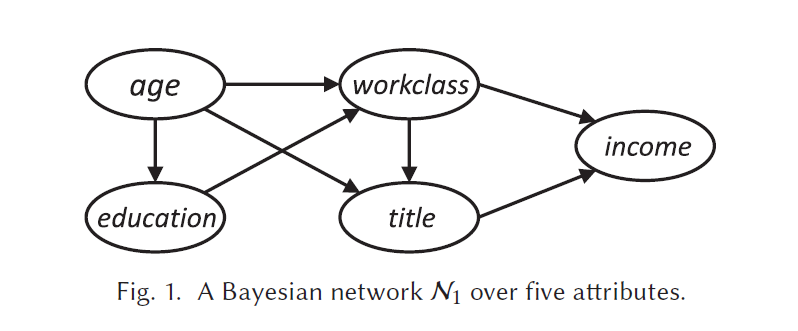
\includegraphics[scale=.35]{../graphs/figure_1.PNG}
\end{figure}
\begin{itemize}
    \item In Fig. 1, $\mathcal{N} = 2$, but not known in reality
\end{itemize}
}

% \frame{\frametitle{Efficiency - Duration (in seconds)}
% \vskip -2mm
% \begin{table}[!h]
%     \centering
%     \rowcolors{1}{white}{lightgray}
%     \resizebox{\textwidth}{!}{% latex table generated in R 4.4.0 by xtable 1.8-4 package
% Fri Jul 19 16:14:31 2024
\begin{tabular}{llrrrr}
  \toprule
version & description & ctgan & datasynthesizer & synthpop (csv) & synthpop (package) \\ 
  \midrule
v00 & Raw (SD2011) & 331.01 & 245.37 & 2132.12 & 5474.39 \\ 
  v01 & Without eduspec or wkabdur & 290.30 & 264.43 & 10.99 & 8.45 \\ 
  v02 & Without wkabdur & 337.07 & 351.76 & 13.96 & 11.02 \\ 
  v03 & Without eduspec & 306.46 & 351.24 & 11.39 & 8.92 \\ 
  v04 & Last variables: eduspec-wkabdur & 374.57 & 344.02 & 14.23 & 287.85 \\ 
  v05 & Last variables: wkabdur-eduspec & 419.60 & 339.92 & 14.60 & 3657.55 \\ 
  v06 & as.numeric(wkabdur) and last variable: eduspec & 356.02 & 347.36 & 14.12 & 11.05 \\ 
  v07\_1\_20 & + 1 factor variable (20 values) & 339.05 & 264.96 & 42.23 &  \\ 
  v07\_1\_25 & + 1 factor variable (25 values) & 400.28 & 326.84 & 137.47 &  \\ 
  v07\_1\_30 & + 1 factor variable (30 values) & 339.73 & 269.72 & 363.18 &  \\ 
  v07\_2\_20 & + 2 factor variable (20 values) & 369.74 & 339.45 & 74.96 &  \\ 
  v07\_2\_25 & + 2 factor variable (25 values) & 364.56 & 361.81 & 631.43 &  \\ 
  v07\_2\_30 & + 2 factor variable (30 values) & 373.25 & 346.15 & 1222.54 &  \\ 
  v07\_3\_20 & + 3 factor variable (20 values) & 393.99 & 369.58 & 122.77 &  \\ 
  v07\_3\_25 & + 3 factor variable (25 values) & 401.03 & 383.40 & 881.53 &  \\ 
  v07\_3\_30 & + 3 factor variable (30 values) & 394.44 & 424.64 & 3654.59 &  \\ 
   \bottomrule
\end{tabular}
}
%     \label{table_sd2011_duration.tex}
% \end{table}
% }


\frame{\frametitle{SD2011 - pMSE}
\vskip -2mm
\begin{figure}
    \resizebox{.75\textwidth}{!}{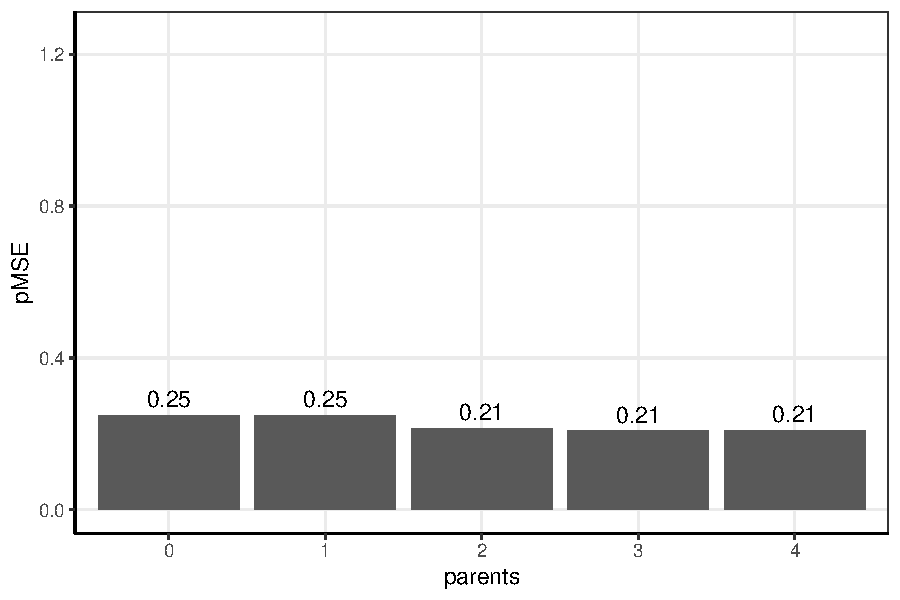
\includegraphics{../graphs/datasynthesizer/datasynthesizer_fidelity_optimize_dataset_parents.pdf}}
    \label{fig:datasynthesizer_fidelity_optimize_dataset_parents}
\end{figure}
}

\frame{\frametitle{DataSynthesizer - SD2011(a)}
\vskip -2mm
\begin{figure}
    \resizebox{.75\textwidth}{!}{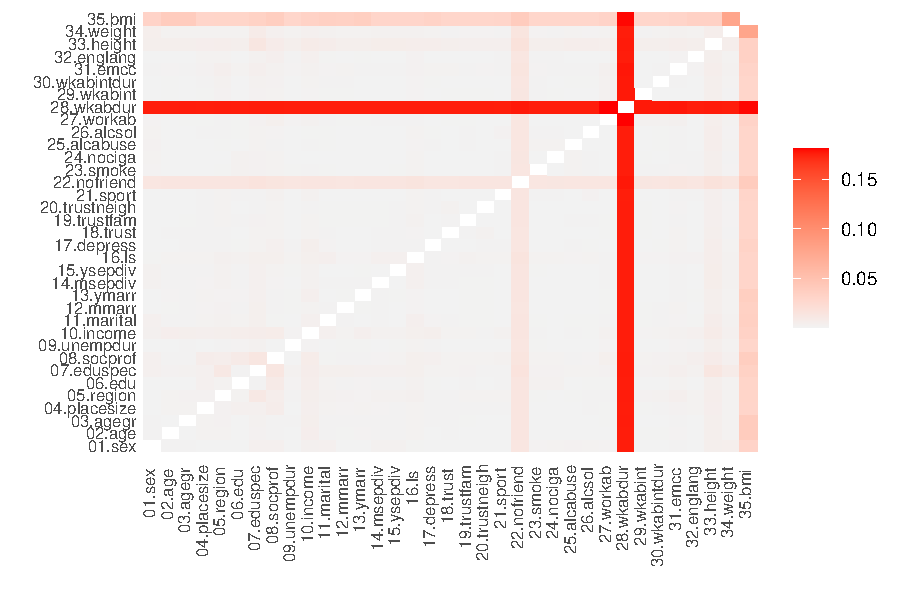
\includegraphics{../graphs/datasynthesizer/datasynthesizer_fidelity_twoway_sd2011_presentation.pdf}}
    \label{fig:ds_fidelity_two_way_subfig-a}
\end{figure}
}

\frame{\frametitle{variable: wkabdur (Work abroad duration)}
\vskip -2mm
\begin{figure}
    \resizebox{.75\textwidth}{!}{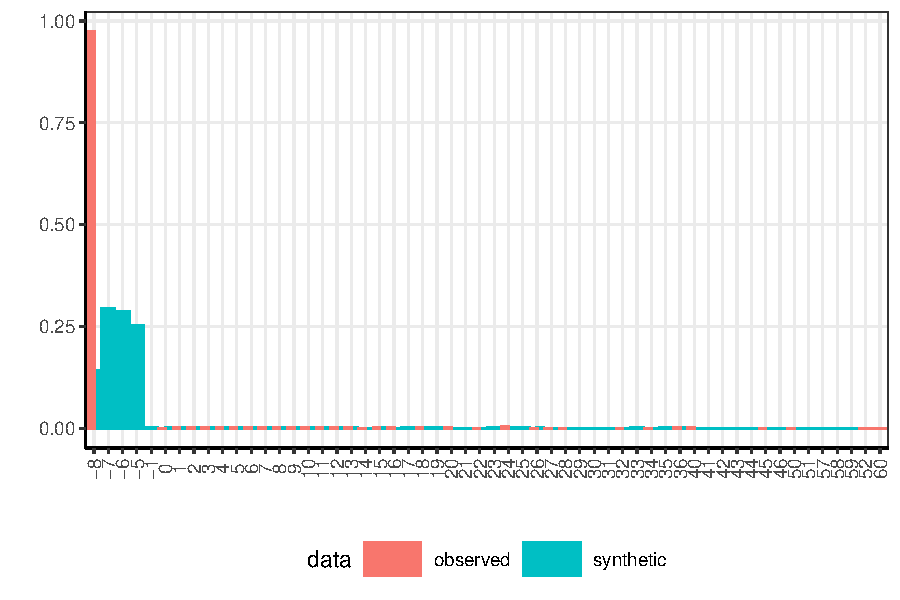
\includegraphics{../graphs/datasynthesizer/datasynthesizer_wkabdur.pdf}}
    \label{fig:ds_variable_wkabdur}
\end{figure}
}

\frame{\frametitle{DataSynthesizer - SD2011(b)}
\vskip -2mm
\begin{figure}
    \resizebox{.75\textwidth}{!}{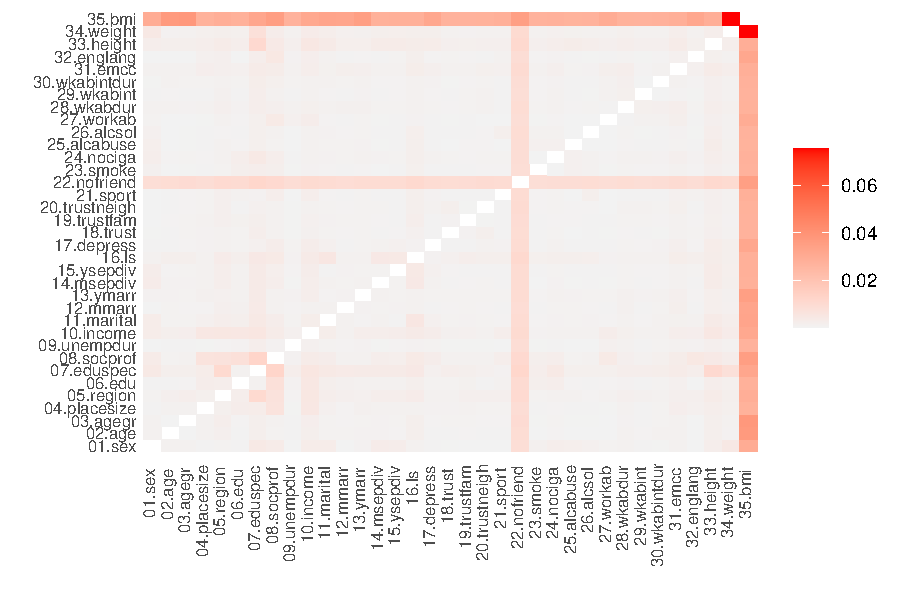
\includegraphics{../graphs/datasynthesizer/datasynthesizer_fidelity_twoway_sd2011_clean_presentation.pdf}}
    \label{fig:ds_fidelity_two_way_subfig-b}
\end{figure}
}

\frame{\frametitle{variable: bmi}
\vskip -2mm
\begin{figure}
    \caption{BMI $<$ 20 is underweight/malnourished}
\vskip -2mm
    \resizebox{.7\textwidth}{!}{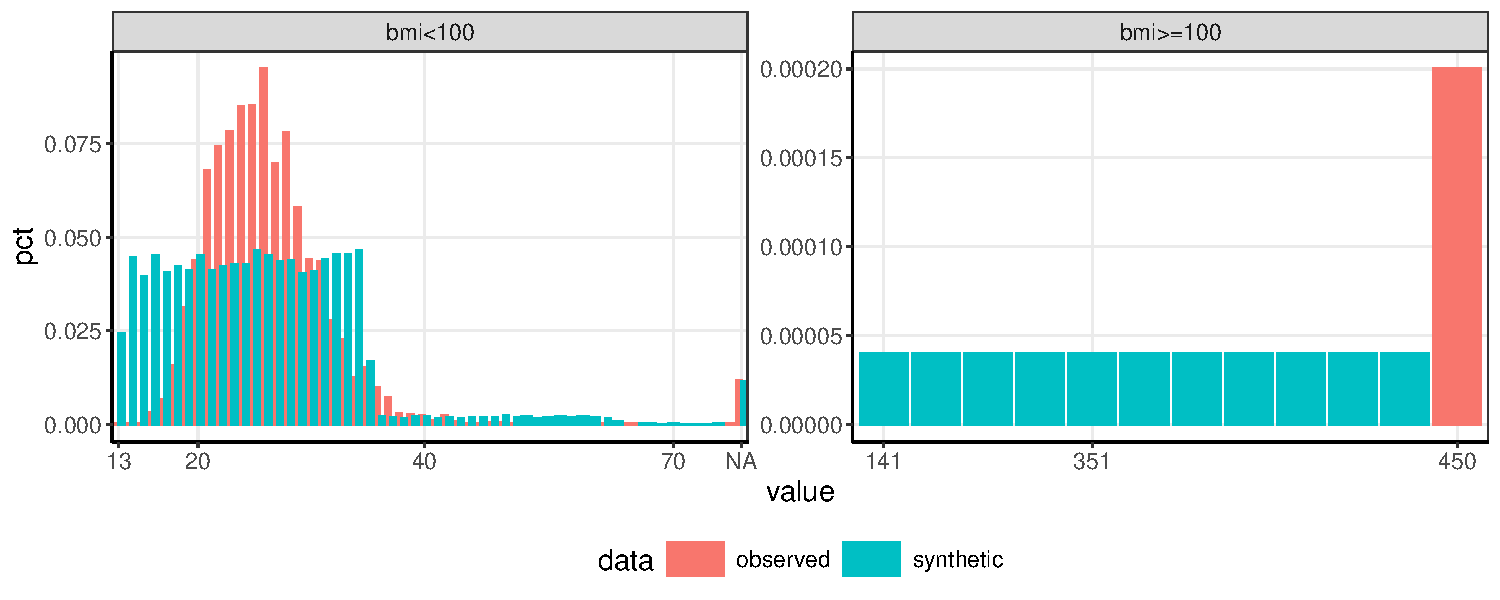
\includegraphics{../graphs/datasynthesizer/datasynthesizer_bmi.pdf}}
    \label{fig:ds_variable_bmi}
\end{figure}
}

\frame{\frametitle{DataSynthesizer - SD2011(c)}
\vskip -2mm
\begin{figure}
    \resizebox{.75\textwidth}{!}{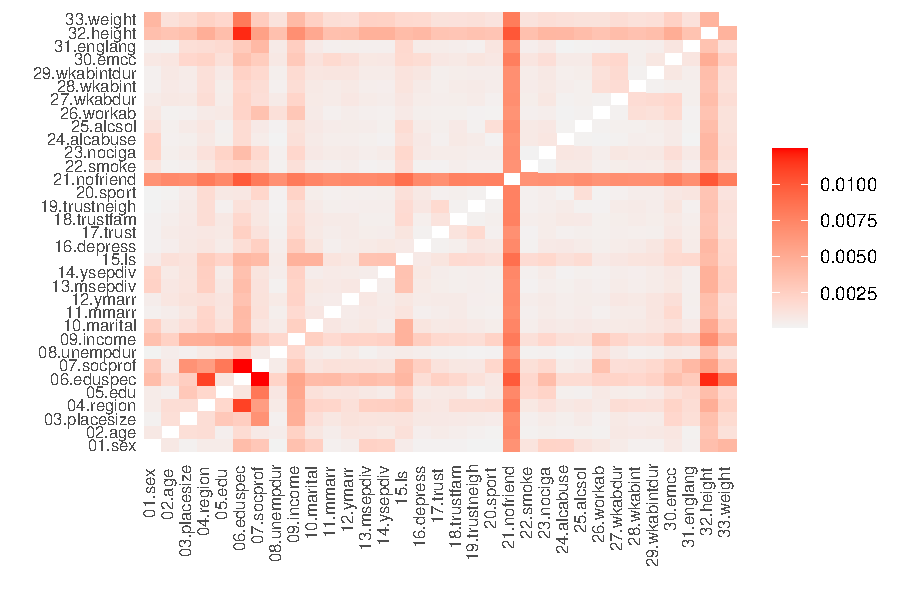
\includegraphics{../graphs/datasynthesizer/datasynthesizer_fidelity_twoway_sd2011_clean_small_presentation.pdf}}
    \label{fig:ds_fidelity_two_way_subfig-c}
\end{figure}
}

\frame{\frametitle{variable: nofriend}
\vskip -2mm
\begin{figure}
    \caption{Doesn't capture rounding/discontinuity}
\vskip -2mm
    \resizebox{.7\textwidth}{!}{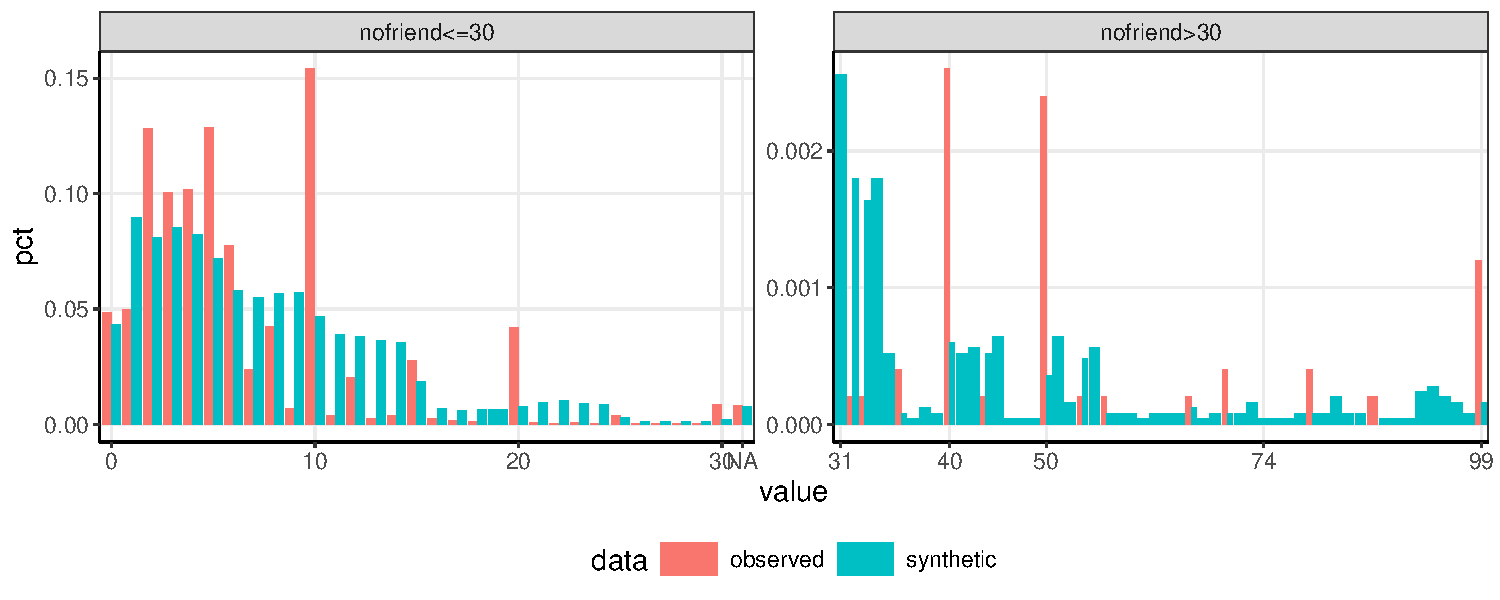
\includegraphics{../graphs/datasynthesizer/datasynthesizer_nofriend.pdf}}
    \label{fig:ds_variable_nofriend}
\end{figure}
}

\frame{\frametitle{SD2011 - pMSE}
\vskip -2mm
\begin{figure}
    \resizebox{.75\textwidth}{!}{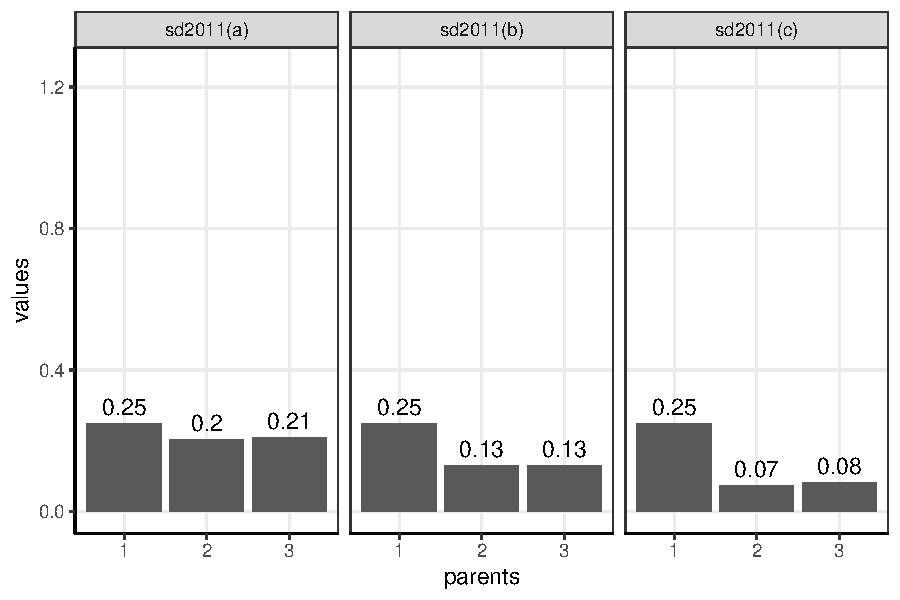
\includegraphics{../graphs/datasynthesizer/datasynthesizer_fidelity_optimize_dataset_parents_compare.pdf}}
    \label{fig:datasynthesizer_fidelity_optimize_dataset_parents_compare}
\end{figure}
}

\frame{\frametitle{Datasynthesizer: selected variables}
\begin{figure}
    \caption{No missings if parents $<$ 2}
    \resizebox{\textwidth}{!}{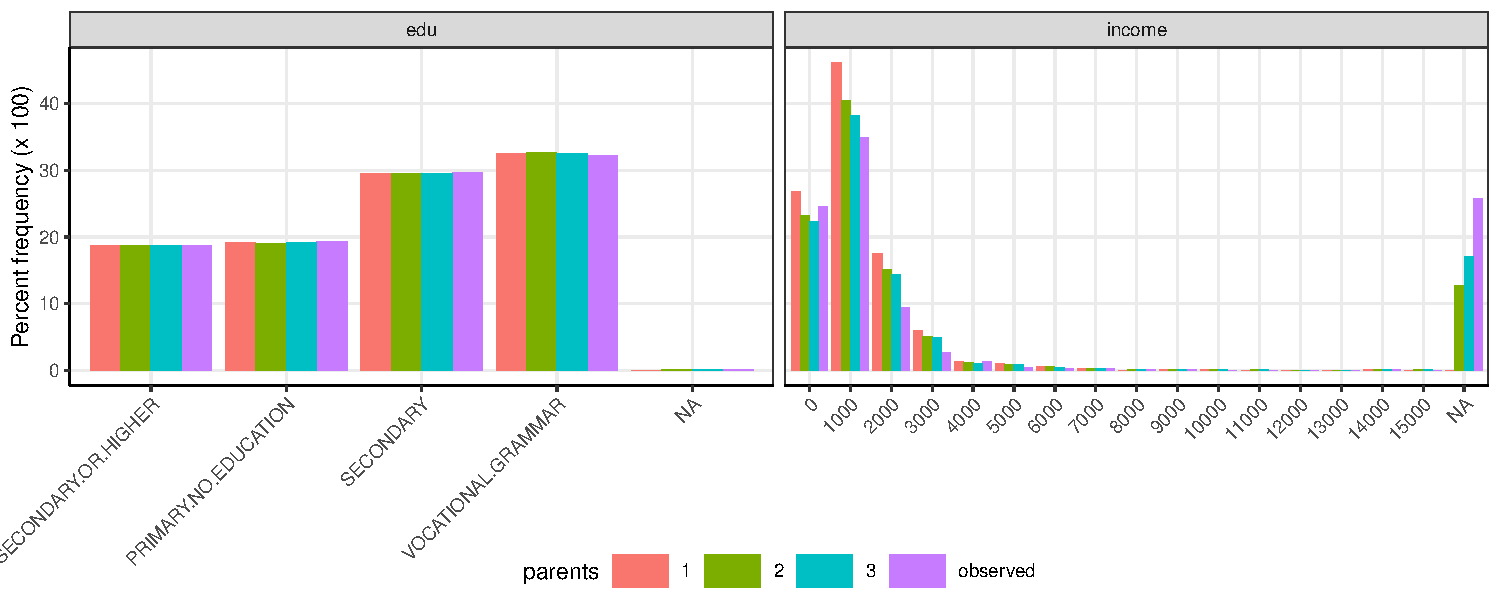
\includegraphics{../graphs/datasynthesizer/datasynthesizer_frequency_optimize_variables_parents.pdf}}
    \label{subfig:tuning_ds_variables_within_synthetic}
\end{figure}
}


\subsection{CTGAN}\label{sec:sdg_ctgan}
\frame[c]{\frametitle{}
\centering
Section \ref{sec:sdg}\ref{sec:sdg_ctgan}: Know your generator (CTGAN)
}

\frame{\frametitle{Tuning CTGAN}
\begin{itemize}
    \item Batch size (constant steps)
    \item Epochs (constant batch size)
    \item Dimensions (2 hyperparameters)
    \begin{itemize}
        \item embedding\_dim (int): Size of the random sample passed to the Generator. Defaults to 128.
        \item dimensionality - 2 hyperparameters, but same value for each
        \begin{itemize}
            \item discriminator\_dim (tuple or list of ints): Size of the output samples for each one of the Discriminator Layers. A Linear Layer will be created for each one of the values provided. Defaults to (256, 256).
            \item generator\_dim (tuple or list of ints): Size of the output samples for each one of the Residuals. A Resiudal Layer will be created for each one of the values provided. Defaults to (256, 256).  
        \end{itemize}
    \end{itemize}
\end{itemize}
}

\frame{\frametitle{Batch size, epochs, and steps}
\begin{table}[!h]
    \rowcolors{1}{white}{lightgray}
    \caption{}
    \centering
    \begin{tabular}{cllll}
    \toprule
    N & Batch size & Steps per Epoch & Epochs & Actual Steps \\
    \midrule
    5.000 & 100 & 50 & 60 & 3,000 \\
    5.000 & 250 & 20 & 150 & 3,000 \\
    5.000 & 500 & 10 & 300 & 3,000 \\
    5.000 & 1.000 & 5 & 600 & 3,000 \\ \hline
    5.000 & 500 & 10 & 100 & 1,000 \\
    5.000 & 500 & 10 & 300 & 3,000 \\
    5.000 & 500 & 10 & 600 & 6,000 \\
    5.000 & 500 & 10 & 900 & 9,000 \\
    \bottomrule
    \end{tabular}
\end{table}
}

% \section{Results}\label{sec:results}
\frame{\frametitle{CTGAN: Effect of batch size (constant steps)}
\begin{figure}
    \resizebox{.75\textwidth}{!}{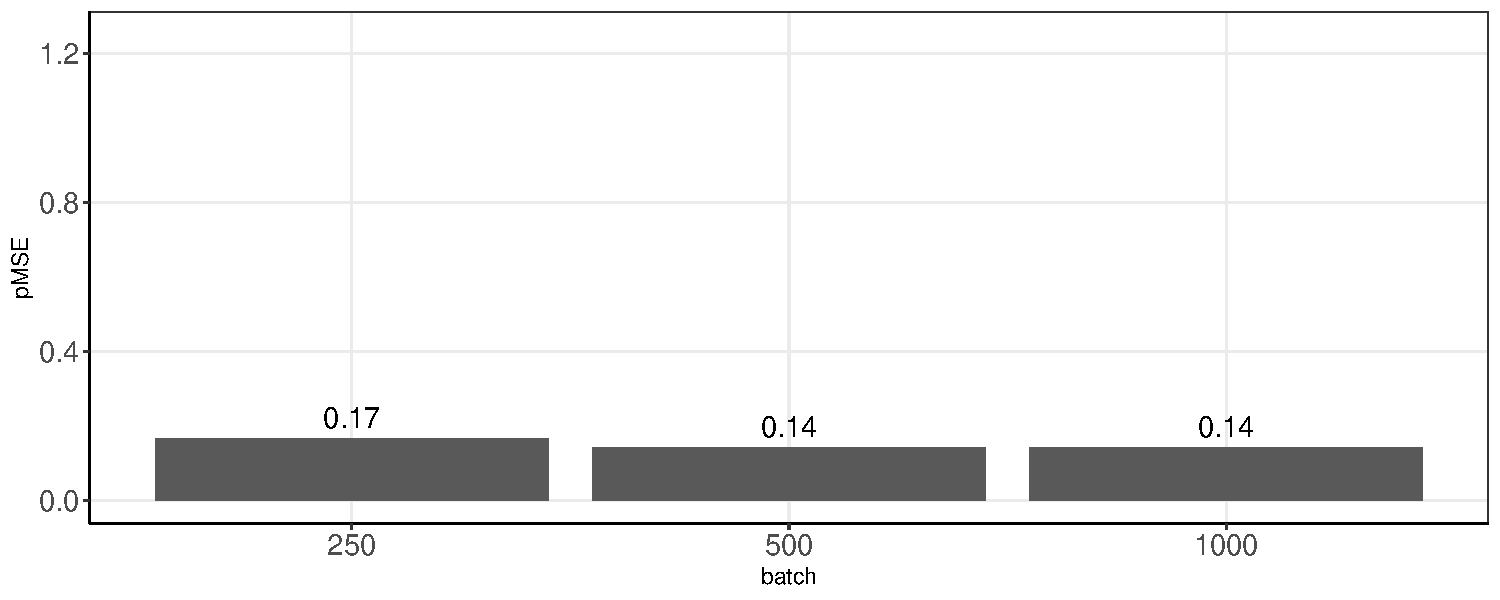
\includegraphics{../../ctgan/graphs/ctgan/ctgan_fidelity_optimize_batch_size.pdf}}
    \label{ctgan_fidelity_optimize_batch_size}
\end{figure}
}

\frame{\frametitle{CTGAN: Effect of epochs (constant batch size)}
\begin{figure}
    \resizebox{.75\textwidth}{!}{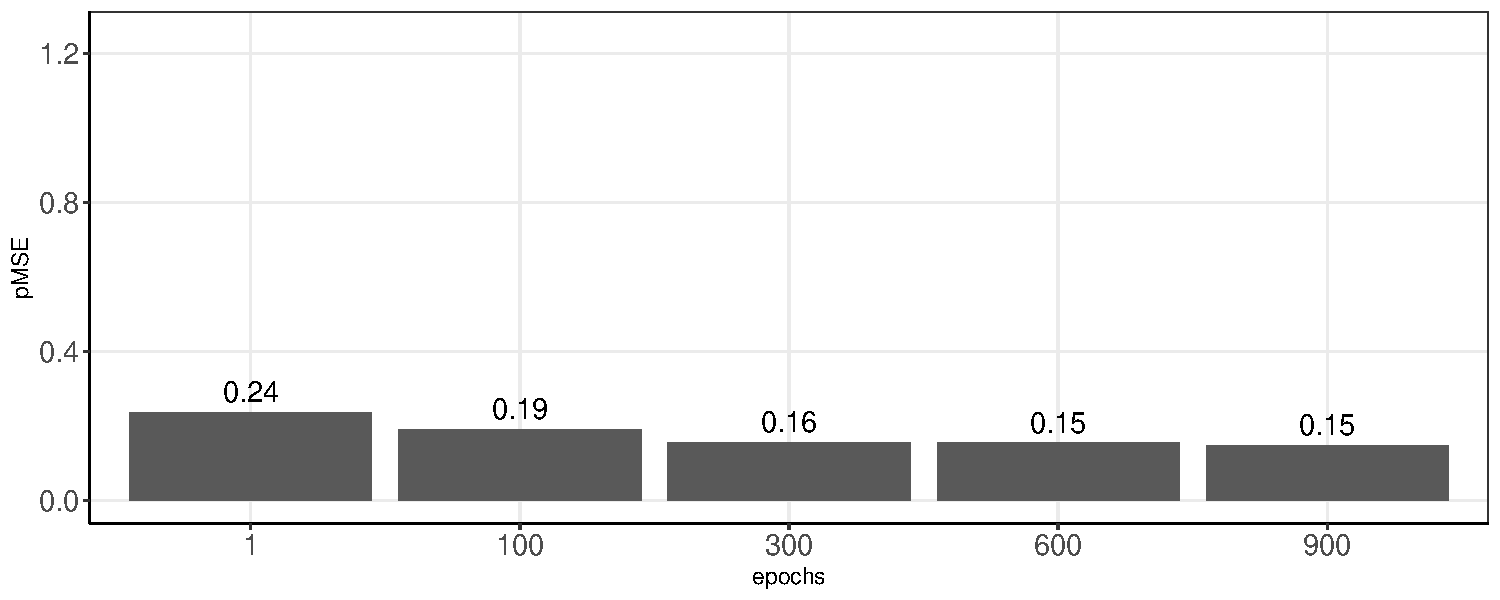
\includegraphics{../../ctgan/graphs/ctgan/ctgan_fidelity_optimize_epochs.pdf}}
    \label{ctgan_fidelity_optimize_epochs}
\end{figure}
}

\frame{\frametitle{CTGAN: Effect of dimensions}
\begin{figure}
    \resizebox{.7\textwidth}{!}{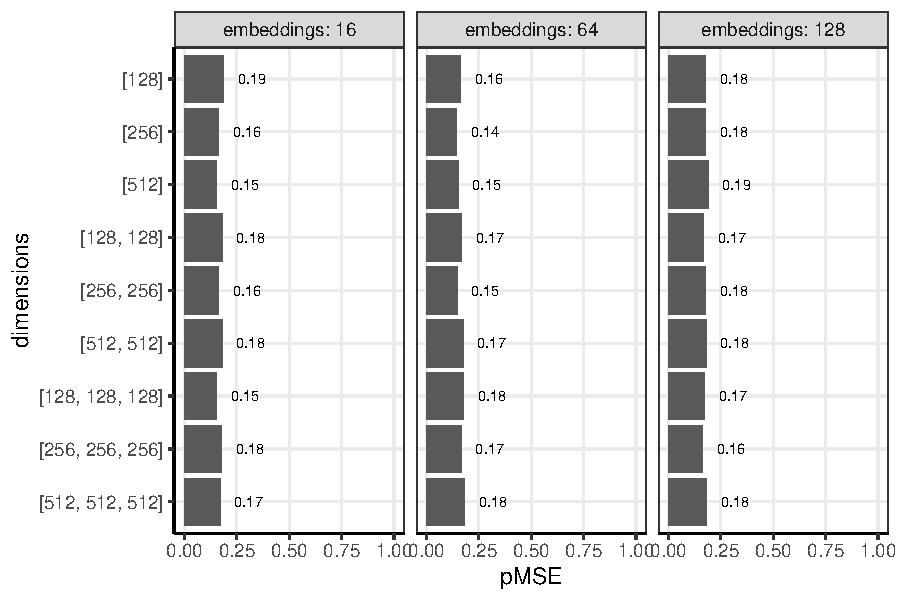
\includegraphics{../../ctgan/graphs/ctgan/ctgan_fidelity_optimize_dimensions.pdf}}
    \label{ctgan_fidelity_optimize_dimensions}
\end{figure}
}

\subsection{Synthpop}\label{sec:sdg_synthpop}
\frame[c]{\frametitle{}
\centering
Section \ref{sec:sdg}\ref{sec:sdg_synthpop}: Know your generator (Synthpop)
}

\frame{\frametitle{Methodology}
According to the online description, Synthpop follows the two-stage process described by Rubin.  

However, if one actually looks at the code, there is an important difference.  

Instead of replacing $y$ with $y^*$ generated by the model, Synthpop replaces $y$ with the leaf number from the regression tree (line 523-523).  

Then, Synthpop predicts the leaf number (line 527) for $y$.  

Finally, Synthpop replaces the predicted leaf number with sampled values of $y$ from the actual data in that leaf (line 549).  

The point: the second-stage replaces values in the synthetic data ($D^*)$ with values in the actual data ($D$).

}



% We are not suggesting that we are revealing some sort of hidden secret.  Even if many users may not be aware, not only is the implementation used in Synthpop based on Reiter \cite{reiter2005using}, it is also well documented in the code with comments.  We do note that the code does not necessarily match with the methodological description, which more generally follows Rubin \cite{rubin1993statistical}.  However, we also believe that one reason why Synthpop has such high levels of utility is because the SDG used in Synthpop samples from the actual data and, related, this implementation does not strictly follow Rubin \cite{rubin1993statistical}.   Therefore, our point is that Synthpop will by definition produce synthetic data sets with higher levels of utility than SDGs that more strictly follow Rubin and only sample from predicted values.\jd{You could make a similar argument for Datasynthesizer if you wanted to. For the categorical variables it also only samples original values. Of course it is true that the low quality of DataSynthesizer partly stems from the fact that it uses a very naive approach to deal with continuous variables, which indeed does not sample original values.}  While Synthpop is a more extreme example, where original observations can theoretically be included in the synthetic data as a result of the mechanism, CART models more generally do not meet definition of Differential Privacy.\jd{I think you can tweak them to be DP. GANs and Bayesian hierarchical models themselves also do not satisfy DP without further tweaking.}


\begin{frame}[fragile]
    \frametitle{Synthpop (syn.cart)}
    \url{https://rdrr.io/cran/synthpop/src/R/functions.syn.r}
    \begin{lstlisting}[language=R]
syn.cart <- function(y, x, xp, smoothing = "", proper = FALSE, 
                     minbucket = 5, cp = 1e-08, ...)
fit <- rpart(y ~ ., data = as.data.frame(cbind(y, x)), method = "anova",
                 minbucket = minbucket, cp = cp, ...)
# get leaf number for observed data
leafnr  <- floor(as.numeric(row.names(fit$frame[fit$where,])))
# replace yval with leaf number in order to predict later node number 
# rather than yval (mean y for observations classified to a leaf) 
fit$frame$yval <- as.numeric(row.names(fit$frame))
# predict leaf number
nodes       <- predict(object = fit, newdata = xp)

...

uniquenodes <- unique(nodes)
new  <- vector("numeric",nrow(xp))
    for (j in uniquenodes) {
      donors <- y[leafnr == j] # values of y in a leaf
      new[nodes == j] <- resample(donors, size = sum(nodes == j), replace = TRUE)
    }

    \end{lstlisting}
\end{frame}

\frame{\frametitle{Method and code may not be the same}

The code appears to indicate that the synthetic sample is drawn from the observed data in a predicted leaf, rather than the predicted y value.

Is this different than the methodological description?

Does this violate the definition of synthetic data, described above?

{\bf The point (and question): High levels of utility in synthpop may be the result of code that implements the method in a way that is not consistent with the definition of synthetic data}

If true, then utility in Synthpop may be artificially high (which lowers the relative advantage to other data synthesizers)

More research is needed 
}



\section{Conclusion}\label{sec:conclusion}
\frame[c]{\frametitle{}
\centering
Section \ref{sec:conclusion}: Conclusion
}


\end{spacing}
\end{document}

